\section{Projet Unity Pro}

La Figure~\ref{fig:unity_fenetre} est une capture d'écran d'une fenêtre \textit{Unity Pro}. Sur la gauche se trouve l'Arborescence du projet, décrite dans la section suivante et la grande partie à droite est la partie programmation.

\begin{figure}[hbt]
	\centering
	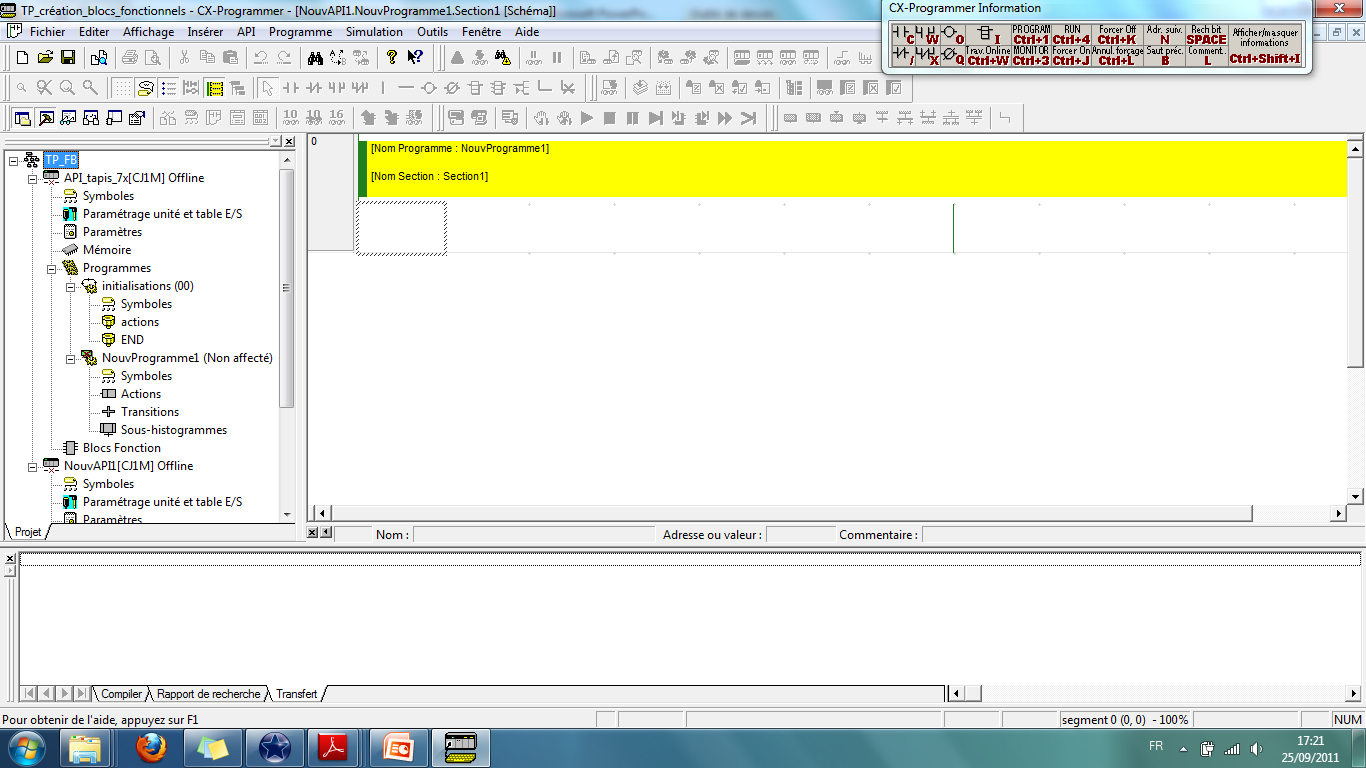
\includegraphics[trim = 0mm 15mm 0mm 0mm, clip,width=.7\linewidth]{images/unity_arbo}
	\caption{Fenêtre Unity Pro}
	\label{fig:unity_fenetre}
\end{figure}

\subsection{L'Arborescence d'un projet Unity}

\begin{figure}[ht]
\centering
\begin{minipage}{.33\linewidth}
	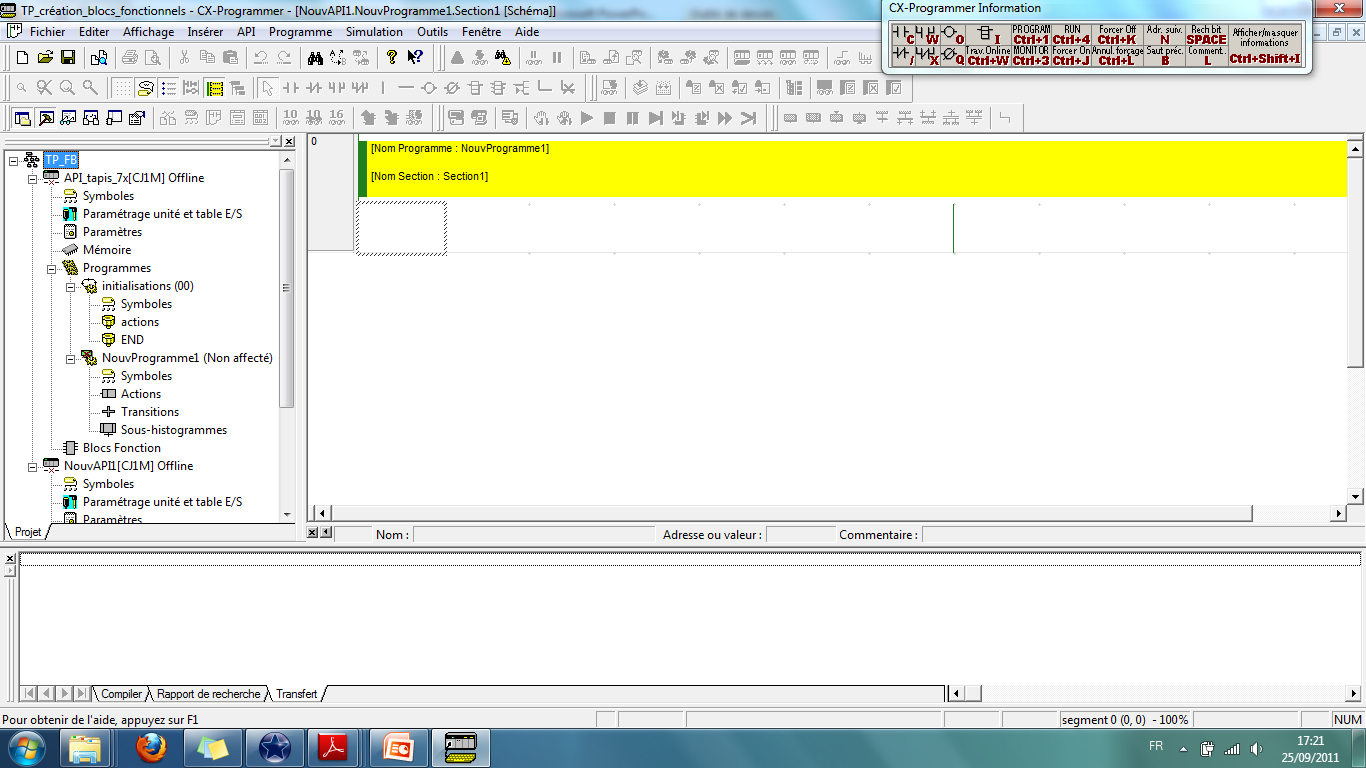
\includegraphics[trim = 2mm 90mm 385mm 53mm, clip, width=\textwidth]{images/unity_arbo}
\end{minipage}\hfill
\begin{minipage}{.63\linewidth}
\dirtree{%
.0 Projet.
.1 API\_Tapis[\dots]/ \DTcomment{Une première configuration}.
	 .2 Symboles \DTcomment{Variables globales}.
	 .2 Paramétrage unité et table E/S.
	 .2 Paramètres \DTcomment{Paramètres de l'automate}.
	 .2 Programmes/ \DTcomment{Programmes dans l'API}.
				.3 Programme\_1/ \DTcomment{Exemple 1 : LADDER}.
					.4 Symboles \DTcomment{Variables locales au programme}.
					.4 actions \DTcomment{Le programme en tant que tel}.
					.4 END.
				.3 Programme\_2/ \DTcomment{Exemple 2 : SFC}.
					.4 Symboles.
					.4 Actions.
					.4 Transitions.
					.4 Sous-histogrammes.
.1 NouvAPI[\dots]/ \DTcomment{Une autre configuration}.
}
\end{minipage}
	\caption{Arborescence d'un projet Unity}
	\label{fig:unity_arbo}
\end{figure}

La Figure~\ref{fig:unity_arbo} présente l'arborescence générale d'un projet \textit{Unity Pro}.

Un projet est constitué de différentes \textbf{configurations} (une configuration pour chaque automate relié au projet). Dans l'exemple de la Figure~\ref{fig:unity_arbo}, les configurations sont 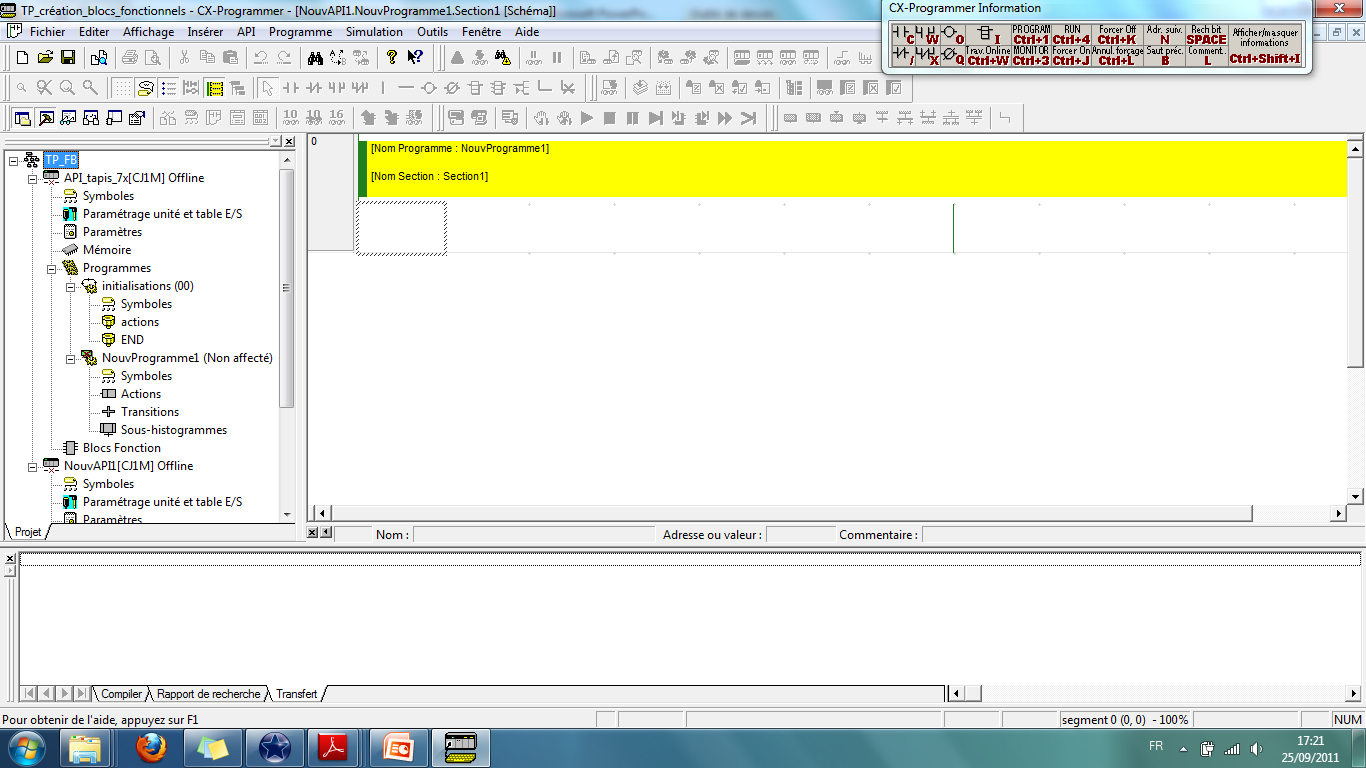
\includegraphics[trim = 40 582 1200 170, clip,height=\fontcharht\font`\B]{images/unity_arbo} et 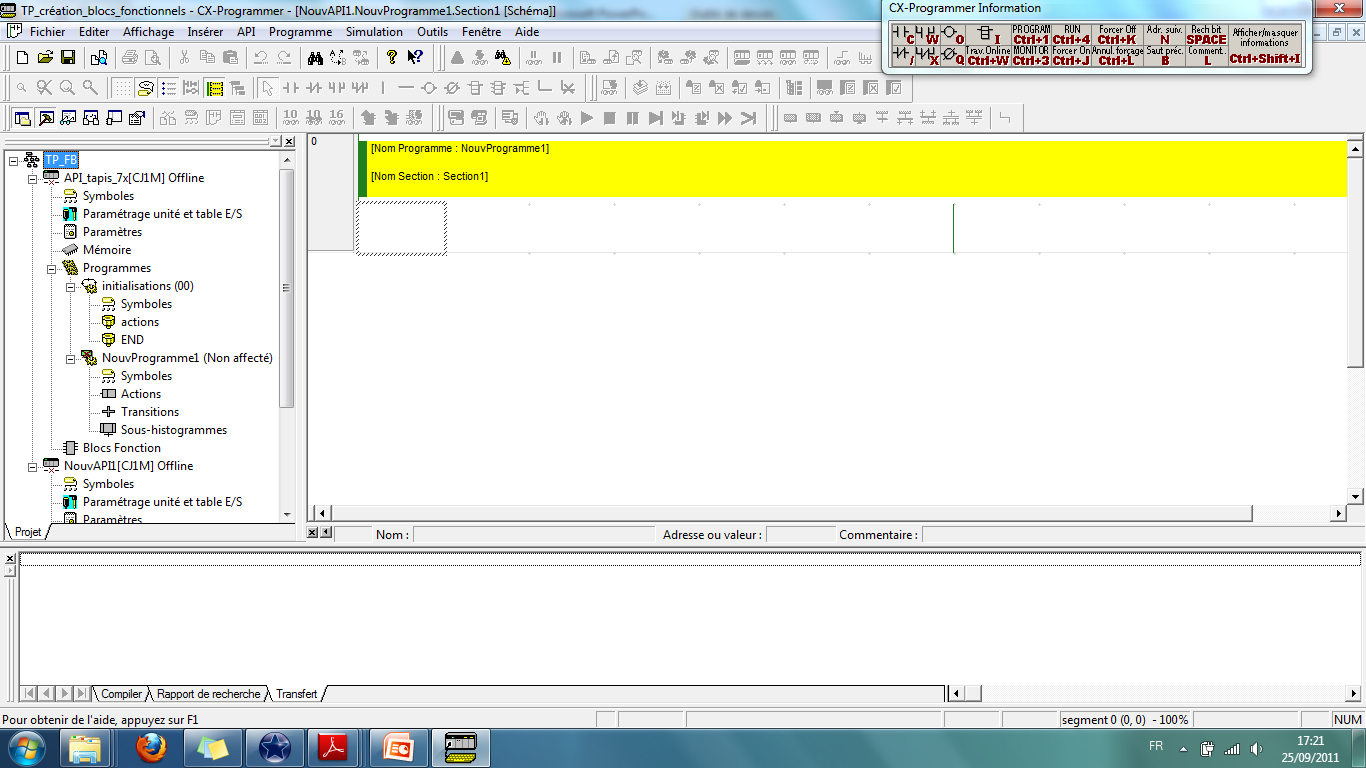
\includegraphics[trim = 40 296 1210 457, clip,height=\fontcharht\font`\B]{images/unity_arbo}.

Dans chaque configuration, on trouve :
\begin{itemize}
	\item Les ressources
		\begin{itemize}
			\item \begin{minipage}[c]{.55\textwidth}
			 	On y trouve la configuration de l'automate, les variables globales (symboles), les déclarations des modules d'entrée-sortie, les registres (mémoire de l'automate) \dots
			\end{minipage}\hfill
			\begin{minipage}[c]{.3\textwidth}
				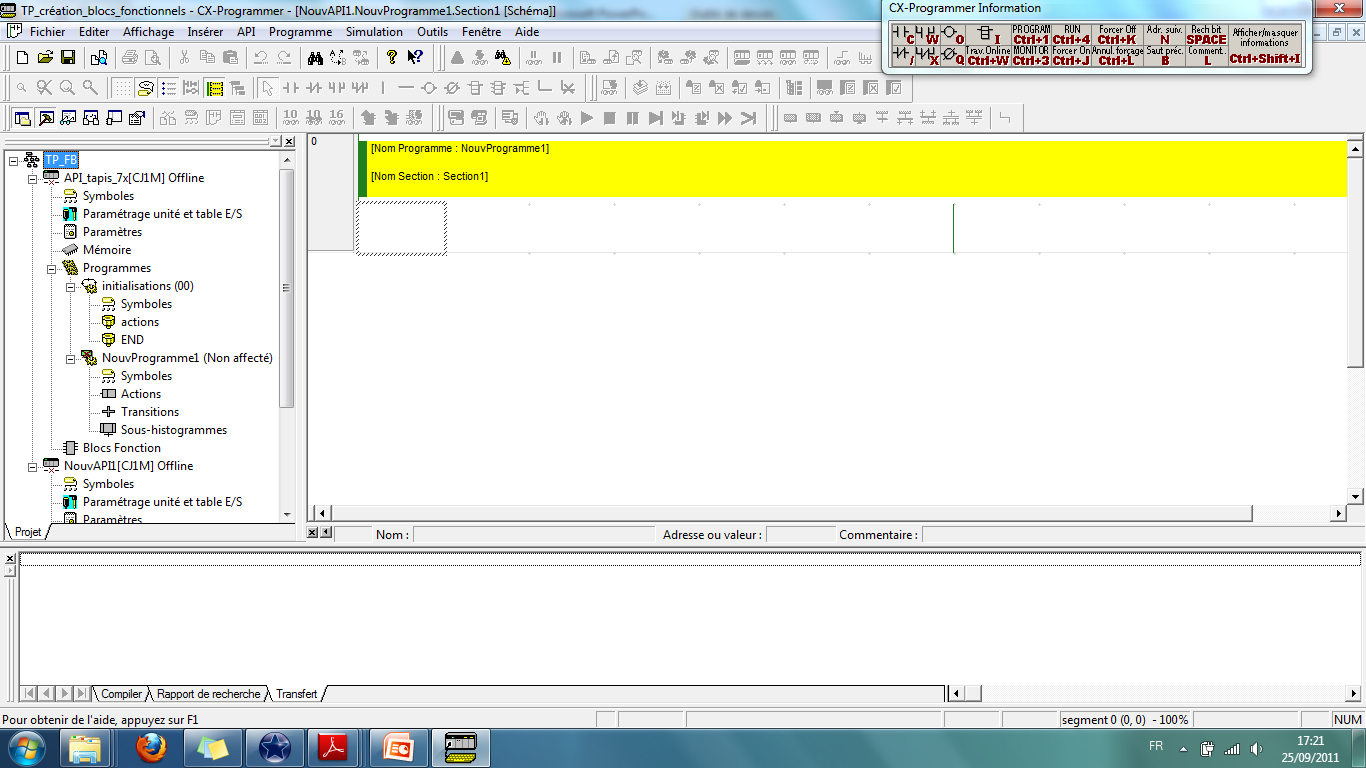
\includegraphics[trim = 50 510 1110 180, clip,height=6\fontcharht\font`\B]{images/unity_arbo}
			\end{minipage}
		\end{itemize}
	\item Les programmes (ou tâche)
	 	\begin{itemize}
		\item tous les programmes d'un automate sont exécutés \textbf{simultanément}
		\item chaque progamme peut avoir des variables locales (symboles)
		\item ils peuvent être écrits en SFC, FBD, LD, ST ou IL.
		\end{itemize}
\end{itemize}
\subsection{Les variables}
Les variables fournissent un moyen d'identifier des objets de données dont le contenu peut varier comme, par exemple, les données associées aux entrées/sorties.

\UPSTIaRetenir{\begin{itemize}
	Les variables sont un moyen de stoquer une donnée (le nombre de pièces dans un bac par exemple) ou de connaître l'état d'un capteur (par exemple la présence d'une pièce devant un capteur ou encore la température)
	\item Les variables (symboles) \textbf{globales} sont utilisables par toutes les tâches
	\item Les variables (symboles) \textbf{locales} à une tâche ne sont utilisables que par cette tâche.
\end{itemize}}

\UPSTIremarque{Dans \textit{Unity Pro}, les variables sont appelées 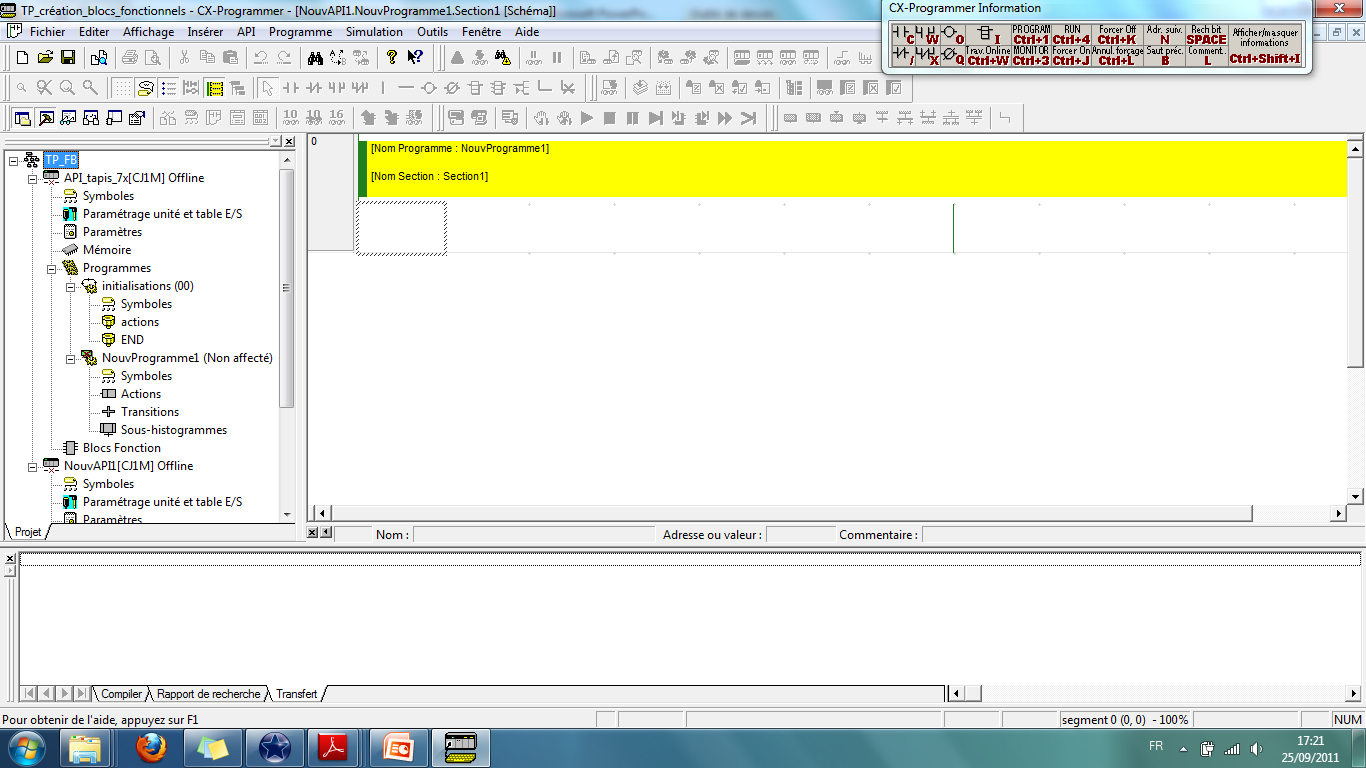
\includegraphics[trim = 100 457.5 1190 298, clip,height=\fontcharht\font`\B]{images/unity_arbo}, on trouve les variables \textbf{globales} dans les ressources de chaque API et les variables locales à chaque programme dans sa propre arborescence.}

Les variables sont donc stoquées dans la mémoire de l'automate. La mémoire d'un automate peut être vue comme une armoire gigantesques composée de différents "tiroirs" dans lesquelles on pourra stoquer une valeur. On représente souvent la mémoire par un tableau dans lequel on stoque une valeur par case. Une variable est donc stoquée dans une des cases du tableau. Le \textit{numéro} de la case est appelé \textbf{adresse} de la variable.

\UPSTIaRetenir[Adresse d'une variable]{
L'\textbf{adresse} d'une variable correspond à l'endroit où cette variable est stoquée dans la mémoire de l'automate.
}

Dans un automate, en plus des variables internes servant à stoquer des infomations, il faut pouvoir accéder aux différentes \textbf{entrées/sorties} de l'automate. Ces entrées/sorties sont également associées à des adresses.

Ces adresses sont d'une forme bien précise : \textbf{\%}\textbf{\color{green}Attribut}\textbf{\color{red}Type}\textbf{\color{blue}k.i.j}. Par exemple : \textbf{\%}\textbf{\color{green} Q}\textbf{\color{red}X}\textbf{\color{blue}2.4.F}.

\begin{table}[hb]
\centering
	\begin{tabular}{l|l|l}
\textbf{\color{green}Attribut}  & \textbf{\color{red}Type} & \textbf{\color{blue}k.j.i}\\%
%
\textbf{I} : Entrée             & \textbf{X} : Booléen      &  \textbf{k} : numéro de voie\\%
\textbf{Q} : Sortie             & \textbf{B} : 8 bits       &  \textbf{j} : numéro de carte\\%
\textbf{M} : Mémoire            & \textbf{W} : 16 bits      &  \textbf{i} : numéro de rack\\%
\textbf{K} : Constante          & \textbf{D} : 32 bits      &  \\%
                               & \textbf{F} : Flottant     &  \\%
\end{tabular} 

	\caption{décomposition d'une adresses}
\end{table}


\subsubsection{Différents types de variables}
En pratique, les variables que l'on stoque n'ont pas toutes le même type et ne nécessite pas la même taille de stockage.

\UPSTIexemple{On comprends aisément qu'un booléen (un seul bit qui ne peut valoir que \textbf{1} ou \textbf{0}) prend moins de place qu'un entier codé sur 8 bits pouvant prendre $2^8$ valeurs.}

Le Tableau~\ref{tab:types_de_donnees} représente les noms et types de données utilisés par les automates.
\begin{table}[h]
	\begin{tabular}{llcc}
\textbf{Nom} & \textbf{Type de données} & \textbf{Taille (bits)} & \textbf{Plage de valeurs}\\\hline
Boolean        & \textbf{BOOL}   & 1   &  0 (faux) ou 1 (vrai) \\\hline\hline%
%
Short integer  & \textbf{SINT}   & 8   &  $[-128 ; 127]$ \\\hline
Integer        & \textbf{INT}    & 16  &  $[-32768 ; 32767]$ \\\hline
Double interger& \textbf{DINT}   & 32  &  $[-2 147 483 648 ; 2 147 483 647]$ \\\hline\hline%
%
Unsigned Short integer  & \textbf{USINT}   & 8   &  $[0 ; 255]$ \\\hline
Unsigned Integer        & \textbf{UINT}    & 16  &  $[0 ; 65535]$ \\\hline
Unsigned Double interger& \textbf{UDINT}   & 32  &  $[0 ; 4294967295]$ \\\hline\hline%
%
Real number  & \textbf{REAL}   &  32   & $[-2^128 ; 2^128]$  \\\hline\hline%
%
Bit string of length 8  & \textbf{BYTE}   &   8  &  $[00 ; FF]$ \\\hline
Bit string of length 16  & \textbf{WORD}   &   16  &  $[0000 ; FFFF]$ \\\hline
Bit string of length 32  & \textbf{DWORD}   &   32  &  $[0000 ; FFFFFFFF]$ \\\hline\hline%
%
Time & \textbf{TIME} & & 0.0s à 21 474 836.47s \\
\end{tabular}

	\caption{Nom et tailles des différents types de données}
	\label{tab:types_de_donnees}
\end{table}
